\documentclass[10pt, dvipdfmx]{beamer}
\AtBeginDvi{\special{pdf:tounicode 90ms-RKSJ-UCS2}}
\setbeamertemplate{navigation symbols}{}
\usetheme{default}
\setbeamertemplate{footline}[frame number]
\usefonttheme{professionalfonts}
\usepackage{helvet}
\usepackage{moreverb}
\renewcommand{\familydefault}{\sfdefault}
\renewcommand{\kanjifamilydefault}{\gtdefault}
\setbeamertemplate{caption}[numbered]

\title{programming workshop day2}
\author{青木 聖也}
\institute[所属]{多摩美術大学情報デザイン研究室}
\date{August 2, 2017}

\uselanguage{japanese}
\languagepath{japanese}

\begin{document}
    \begin{frame}[plain]
        \frametitle{}
	    \titlepage
    \end{frame}

    \begin{frame}
        \frametitle{Contents}
        \tableofcontents
    \end{frame}

%-----------------------------------------------------------
% 1日目1限:アプリ間通信紹介
    \section{まずはじめに}
        \begin{frame}
            \frametitle{資料について}
            \begin{columns}[c]
                \begin{column}{0.80\textwidth}
                    \begin{block}{今回の資料を以下に公開しています}
                        \begin{itemize}
                            \scriptsize
                            \item 全体説明: http://scottallen.ws/tamabi/summerworkshop2017
                            \item プログラム: https://github.com/5c0tt411en/iddsummerworkshop2017
                            \item スライド: https://github.com/5c0tt411en/iddsummerworkshop2017/blob/master/Slide/
                        \end{itemize}
                    \end{block}
                \end{column}
            \end{columns}
        \end{frame}

    \section{アプリ間通信の作り方}
    \subsection{OSC}
        \begin{frame}
            \frametitle{OSCとは}
            \begin{block}{Open Sound Controlの略アプリ間の通信に使用する形式}
                \begin{itemize}
                    \item URL形式の名前付け
                    \item 数値やシンボルなど様々な信号を伝達可能
                    \item 遅延少ない
                \end{itemize}
            \end{block}
        \end{frame}

        \begin{frame}
            \frametitle{OSCの使用事例1 マシン間での映像同期}
                \begin{figure}[htb]
                    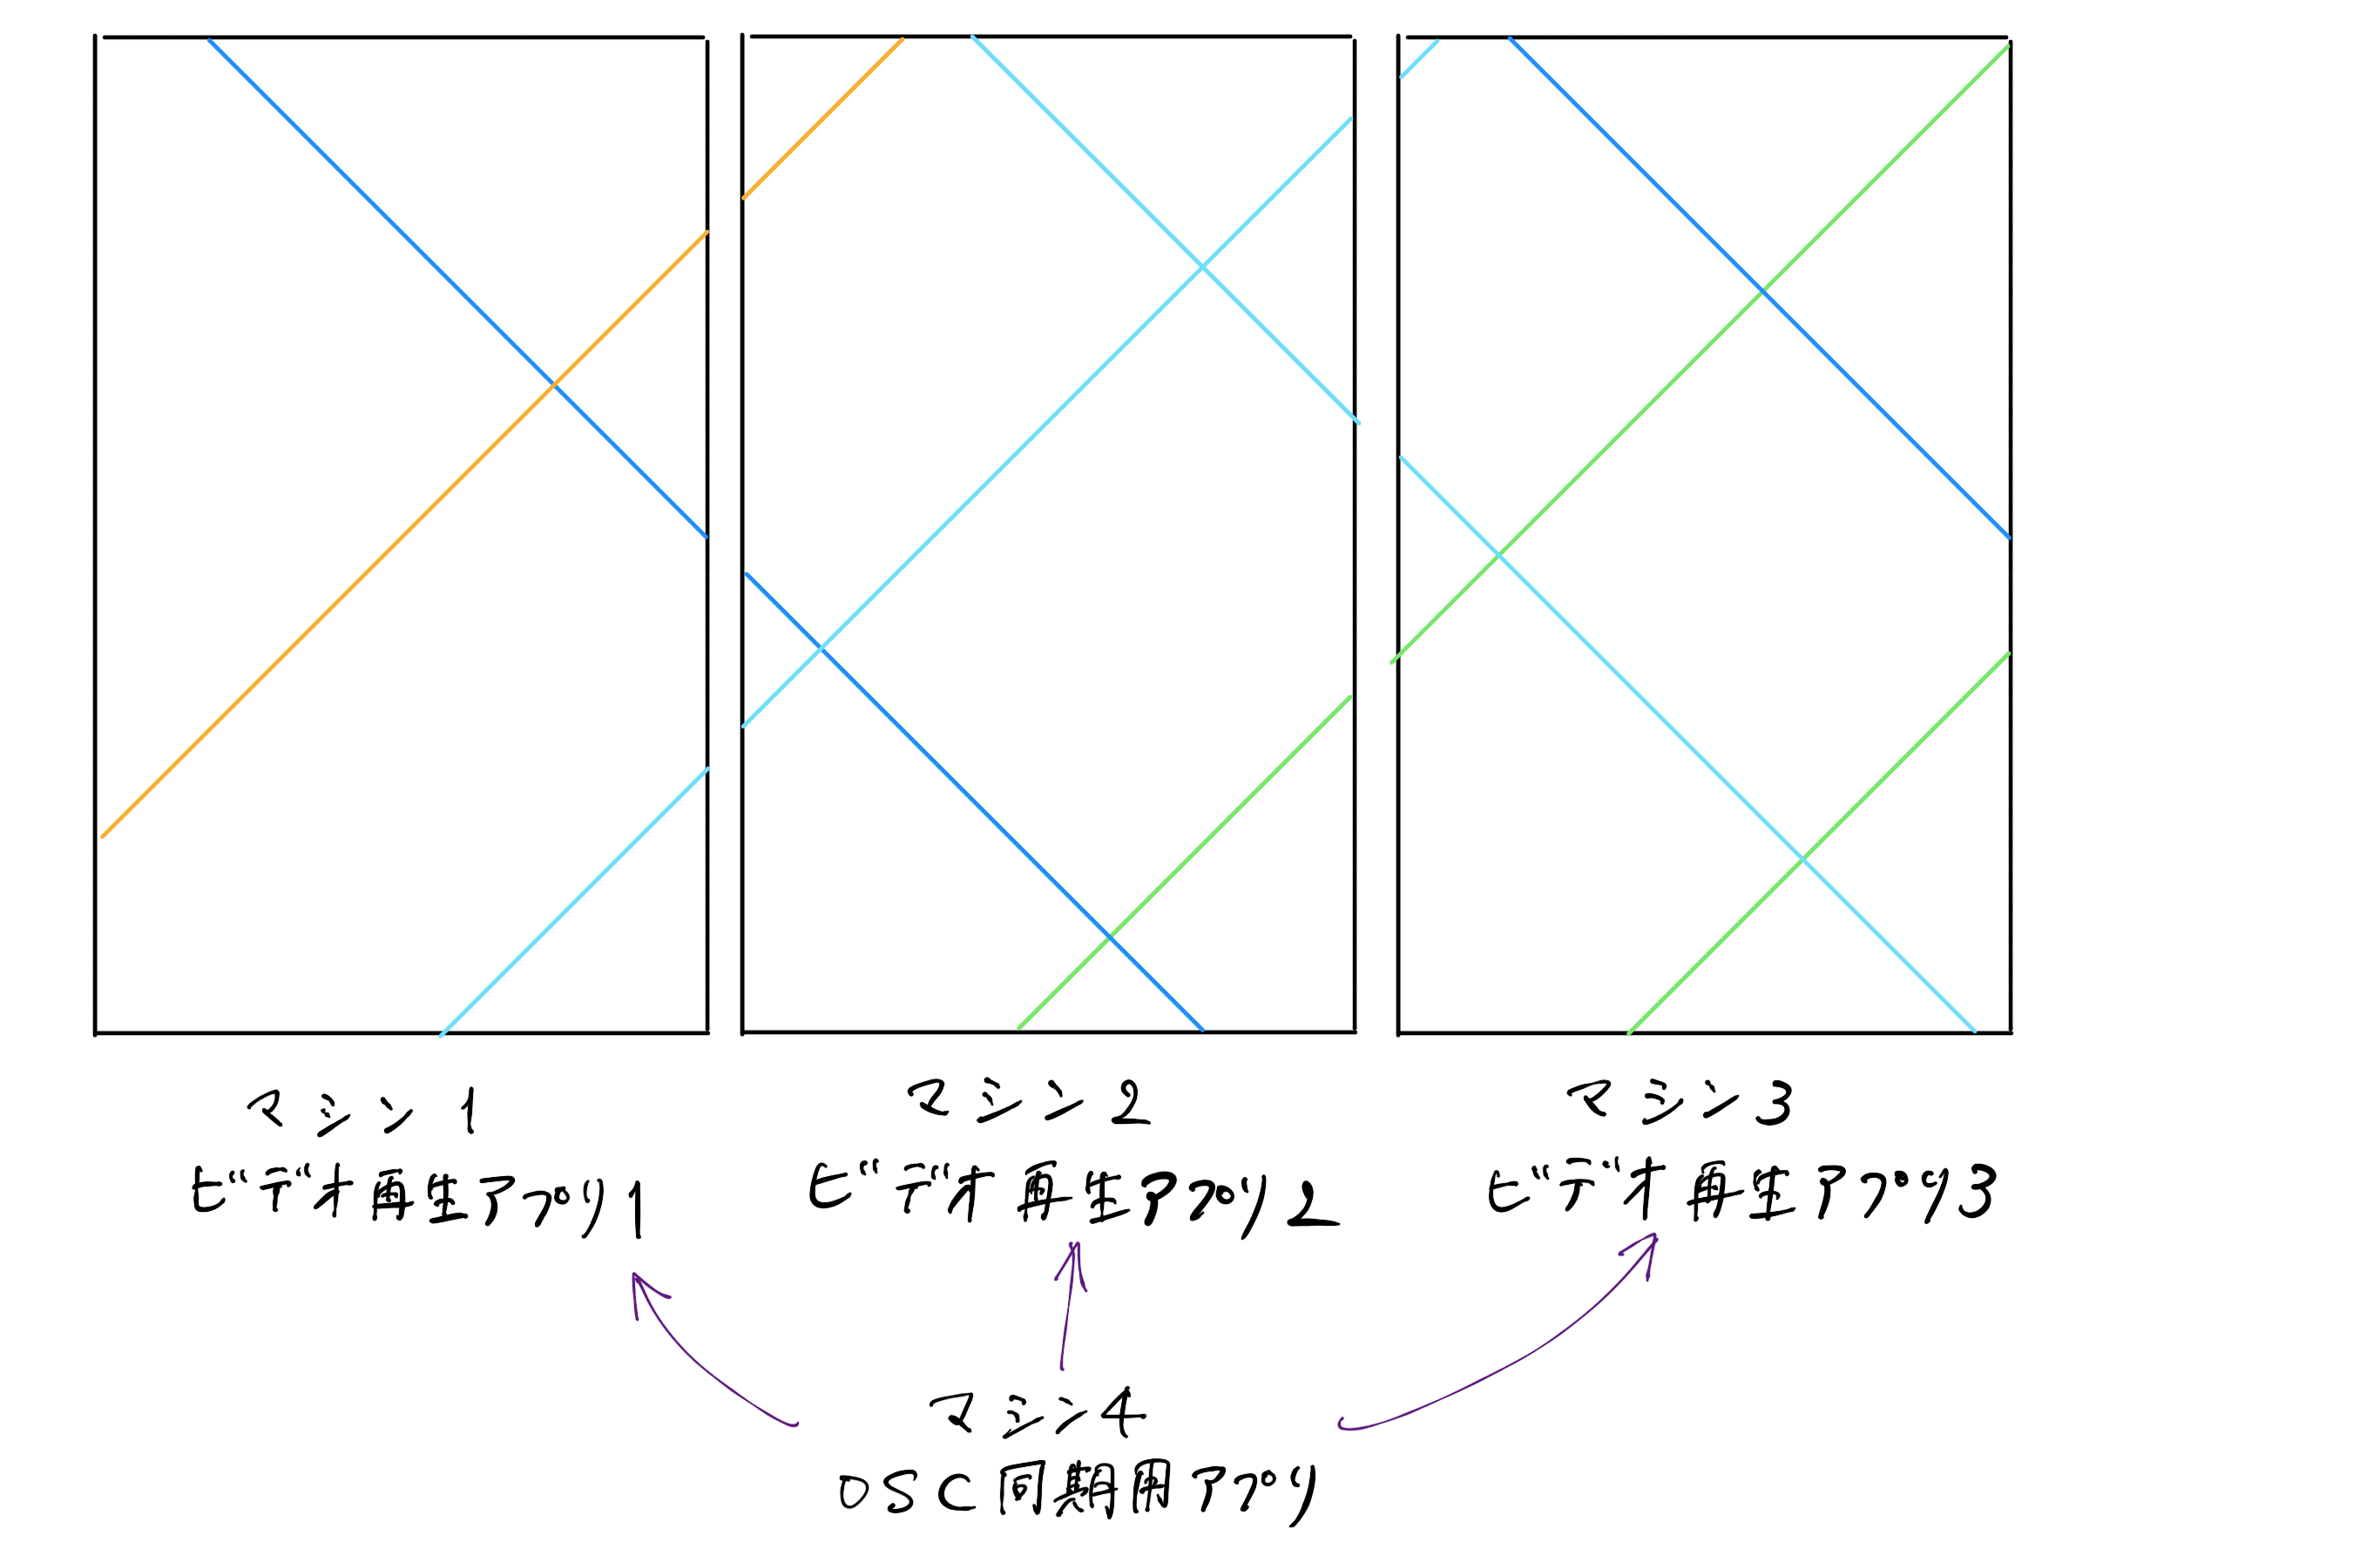
\includegraphics[width=100mm]{images/osc-1.png}
                    \caption{マシン間での映像同期参考図}
                    \label{fig:01}
                \end{figure}
        \end{frame}

        \begin{frame}
            \frametitle{OSCの使用事例2 アプリ間で座標を渡す}
                \begin{figure}[htb]
                    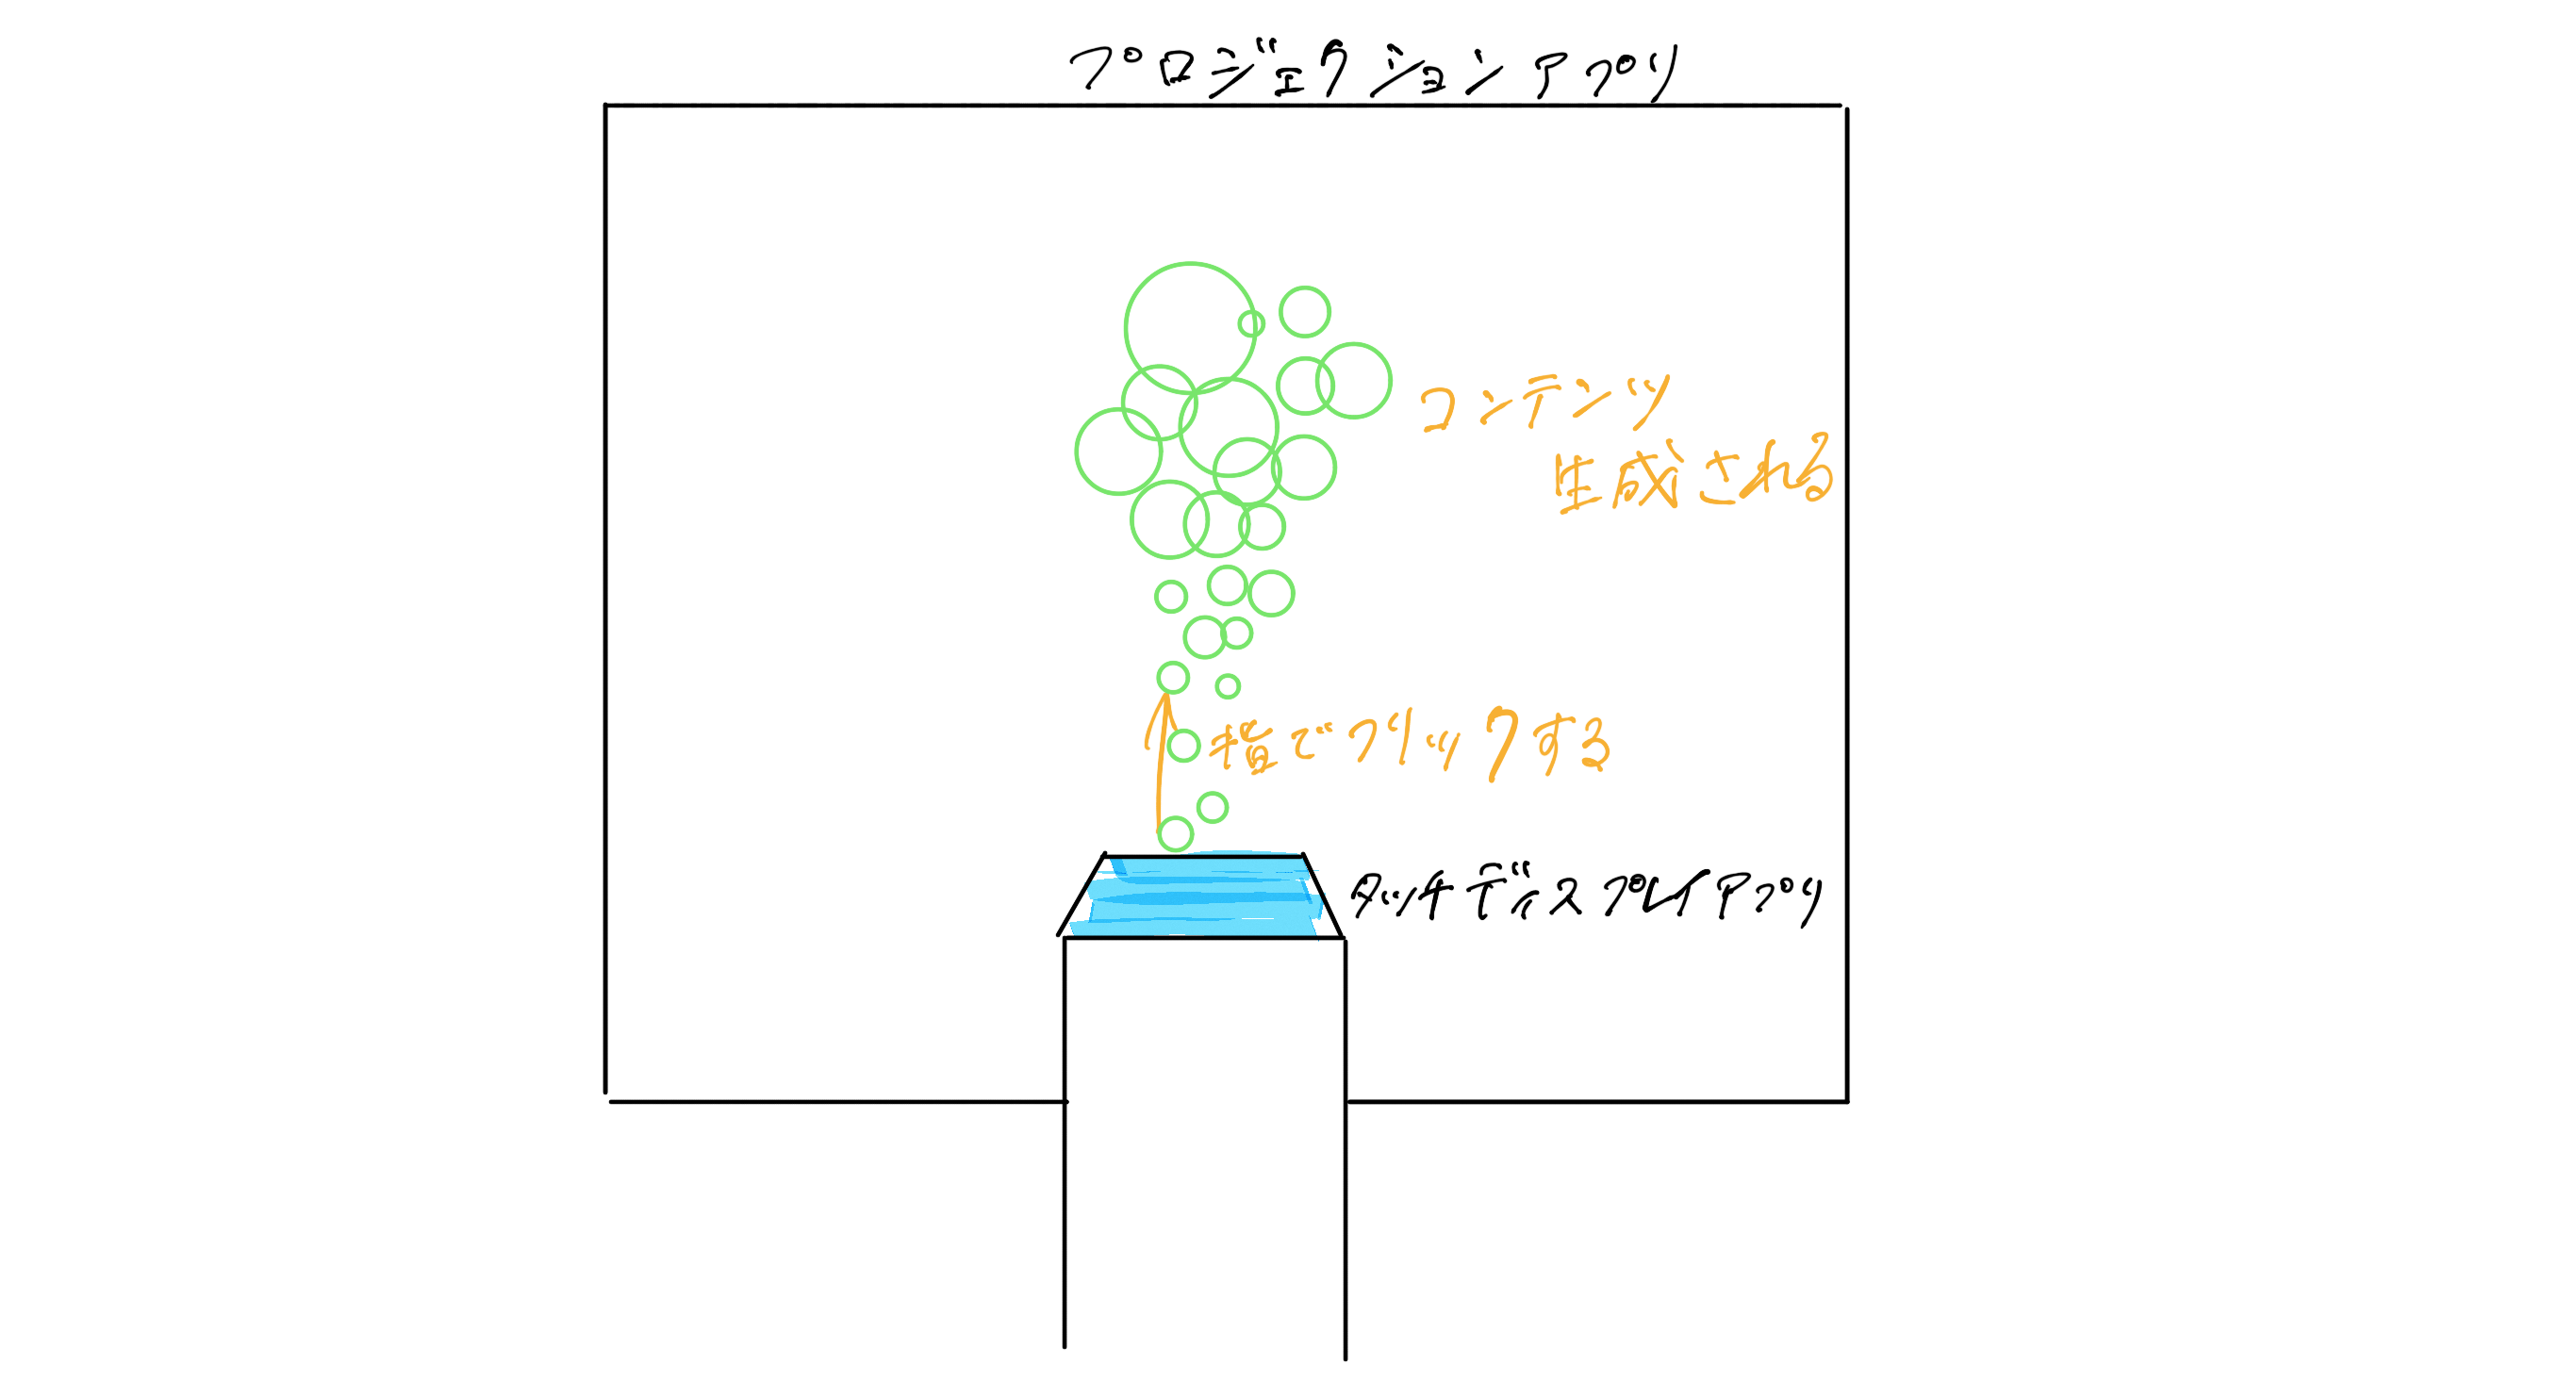
\includegraphics[width=100mm]{images/osc-2.png}
                    \caption{アプリ間で座標を渡す参考図}
                    \label{fig:02}
                \end{figure}
        \end{frame}

    \subsection{信号のやりとり}
        \begin{frame}
            \frametitle{OSCを使った通信方法}
            \begin{block}{送信側}
                \begin{itemize}
                    \item 相手側マシンのipアドレスを指定: 169.254.11.14
                    \item 通信用ポートを指定: 8888
                    \item アドレスを指定: /stat
                    \item 型を明示して値を送信
                \end{itemize}
            \end{block}
            \begin{block}{受信側}
                \begin{itemize}
                    \item 通信用ポートを指定: 8888
                    \item 型を合わせて値を受信
                \end{itemize}
            \end{block}
        \end{frame}

% 1日目2限:openFrameworksを使用した実装
    \subsection{openFrameworksを用いたOSCの送受信}
        \begin{frame}
            \frametitle{OSCを受信する WS06OSCreceiver/}
                \begin{figure}[htb]
                    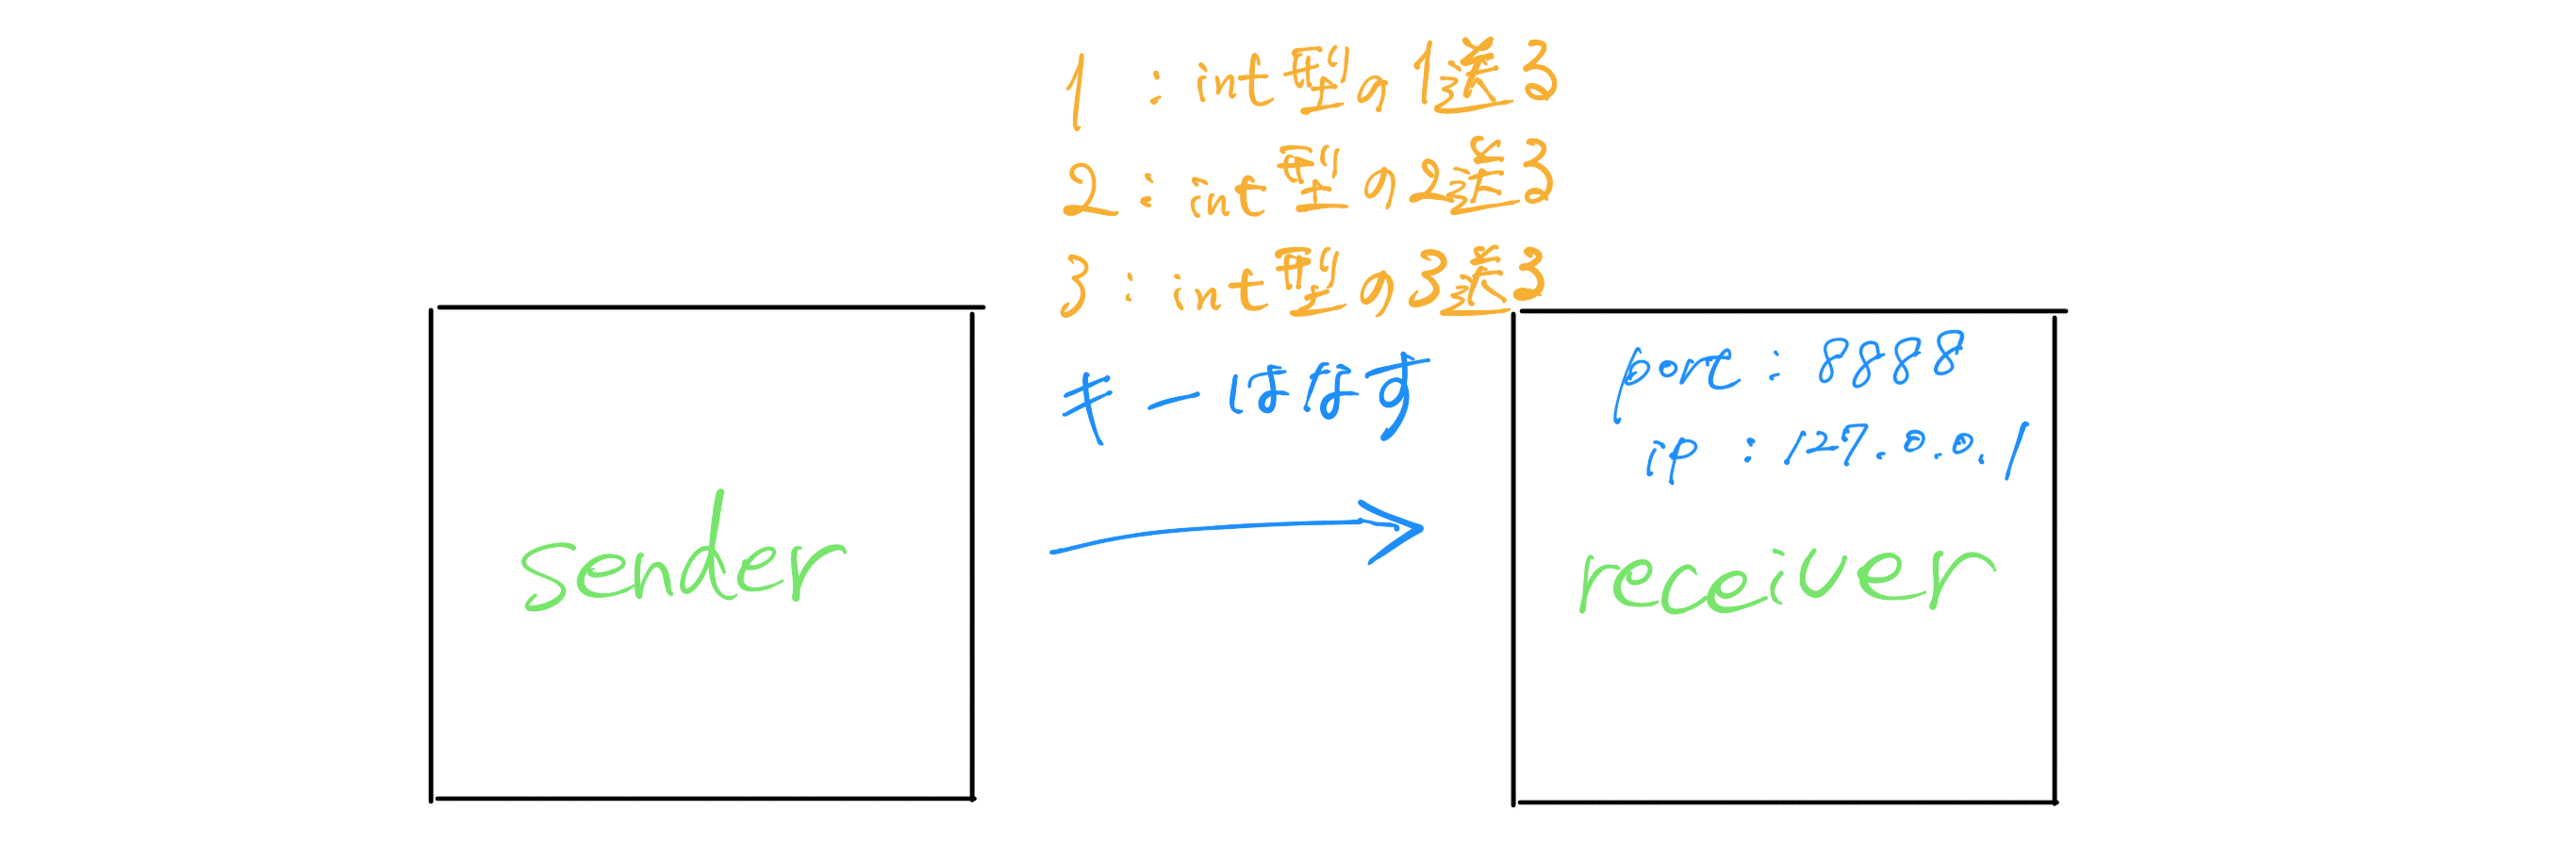
\includegraphics[width=100mm]{images/ws06-1.png}
                    \caption{WS06図解}
                    \label{fig:03}
                \end{figure}
        \end{frame}

        \begin{frame}
            \frametitle{OSCを送信する WS07OSCsender/}
                \begin{figure}[htb]
                    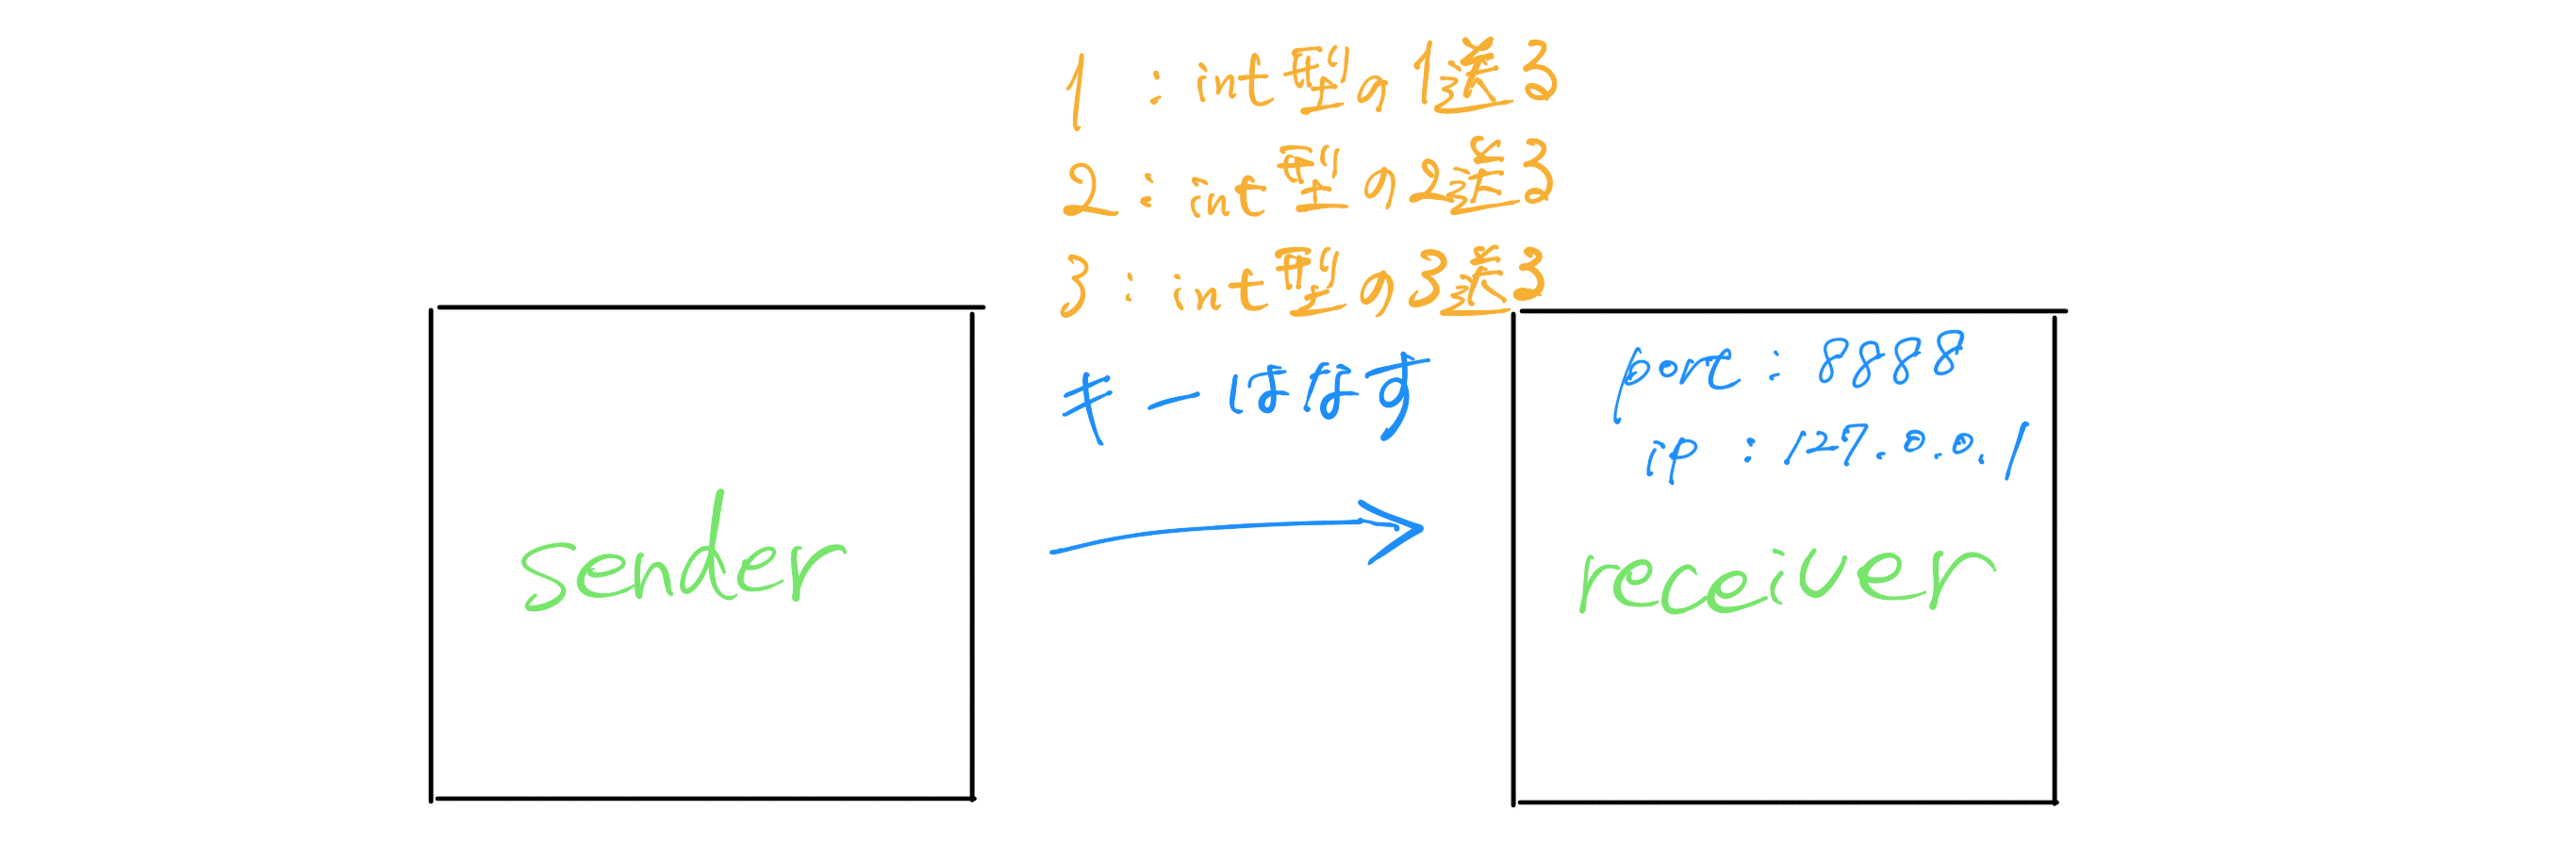
\includegraphics[width=100mm]{images/ws06-1.png}
                    \caption{WS07図解}
                    \label{fig:04}
                \end{figure}
        \end{frame}

        \begin{frame}
            \frametitle{OSCで3面同期 WS08OSCsync/}
                \begin{figure}[htb]
                    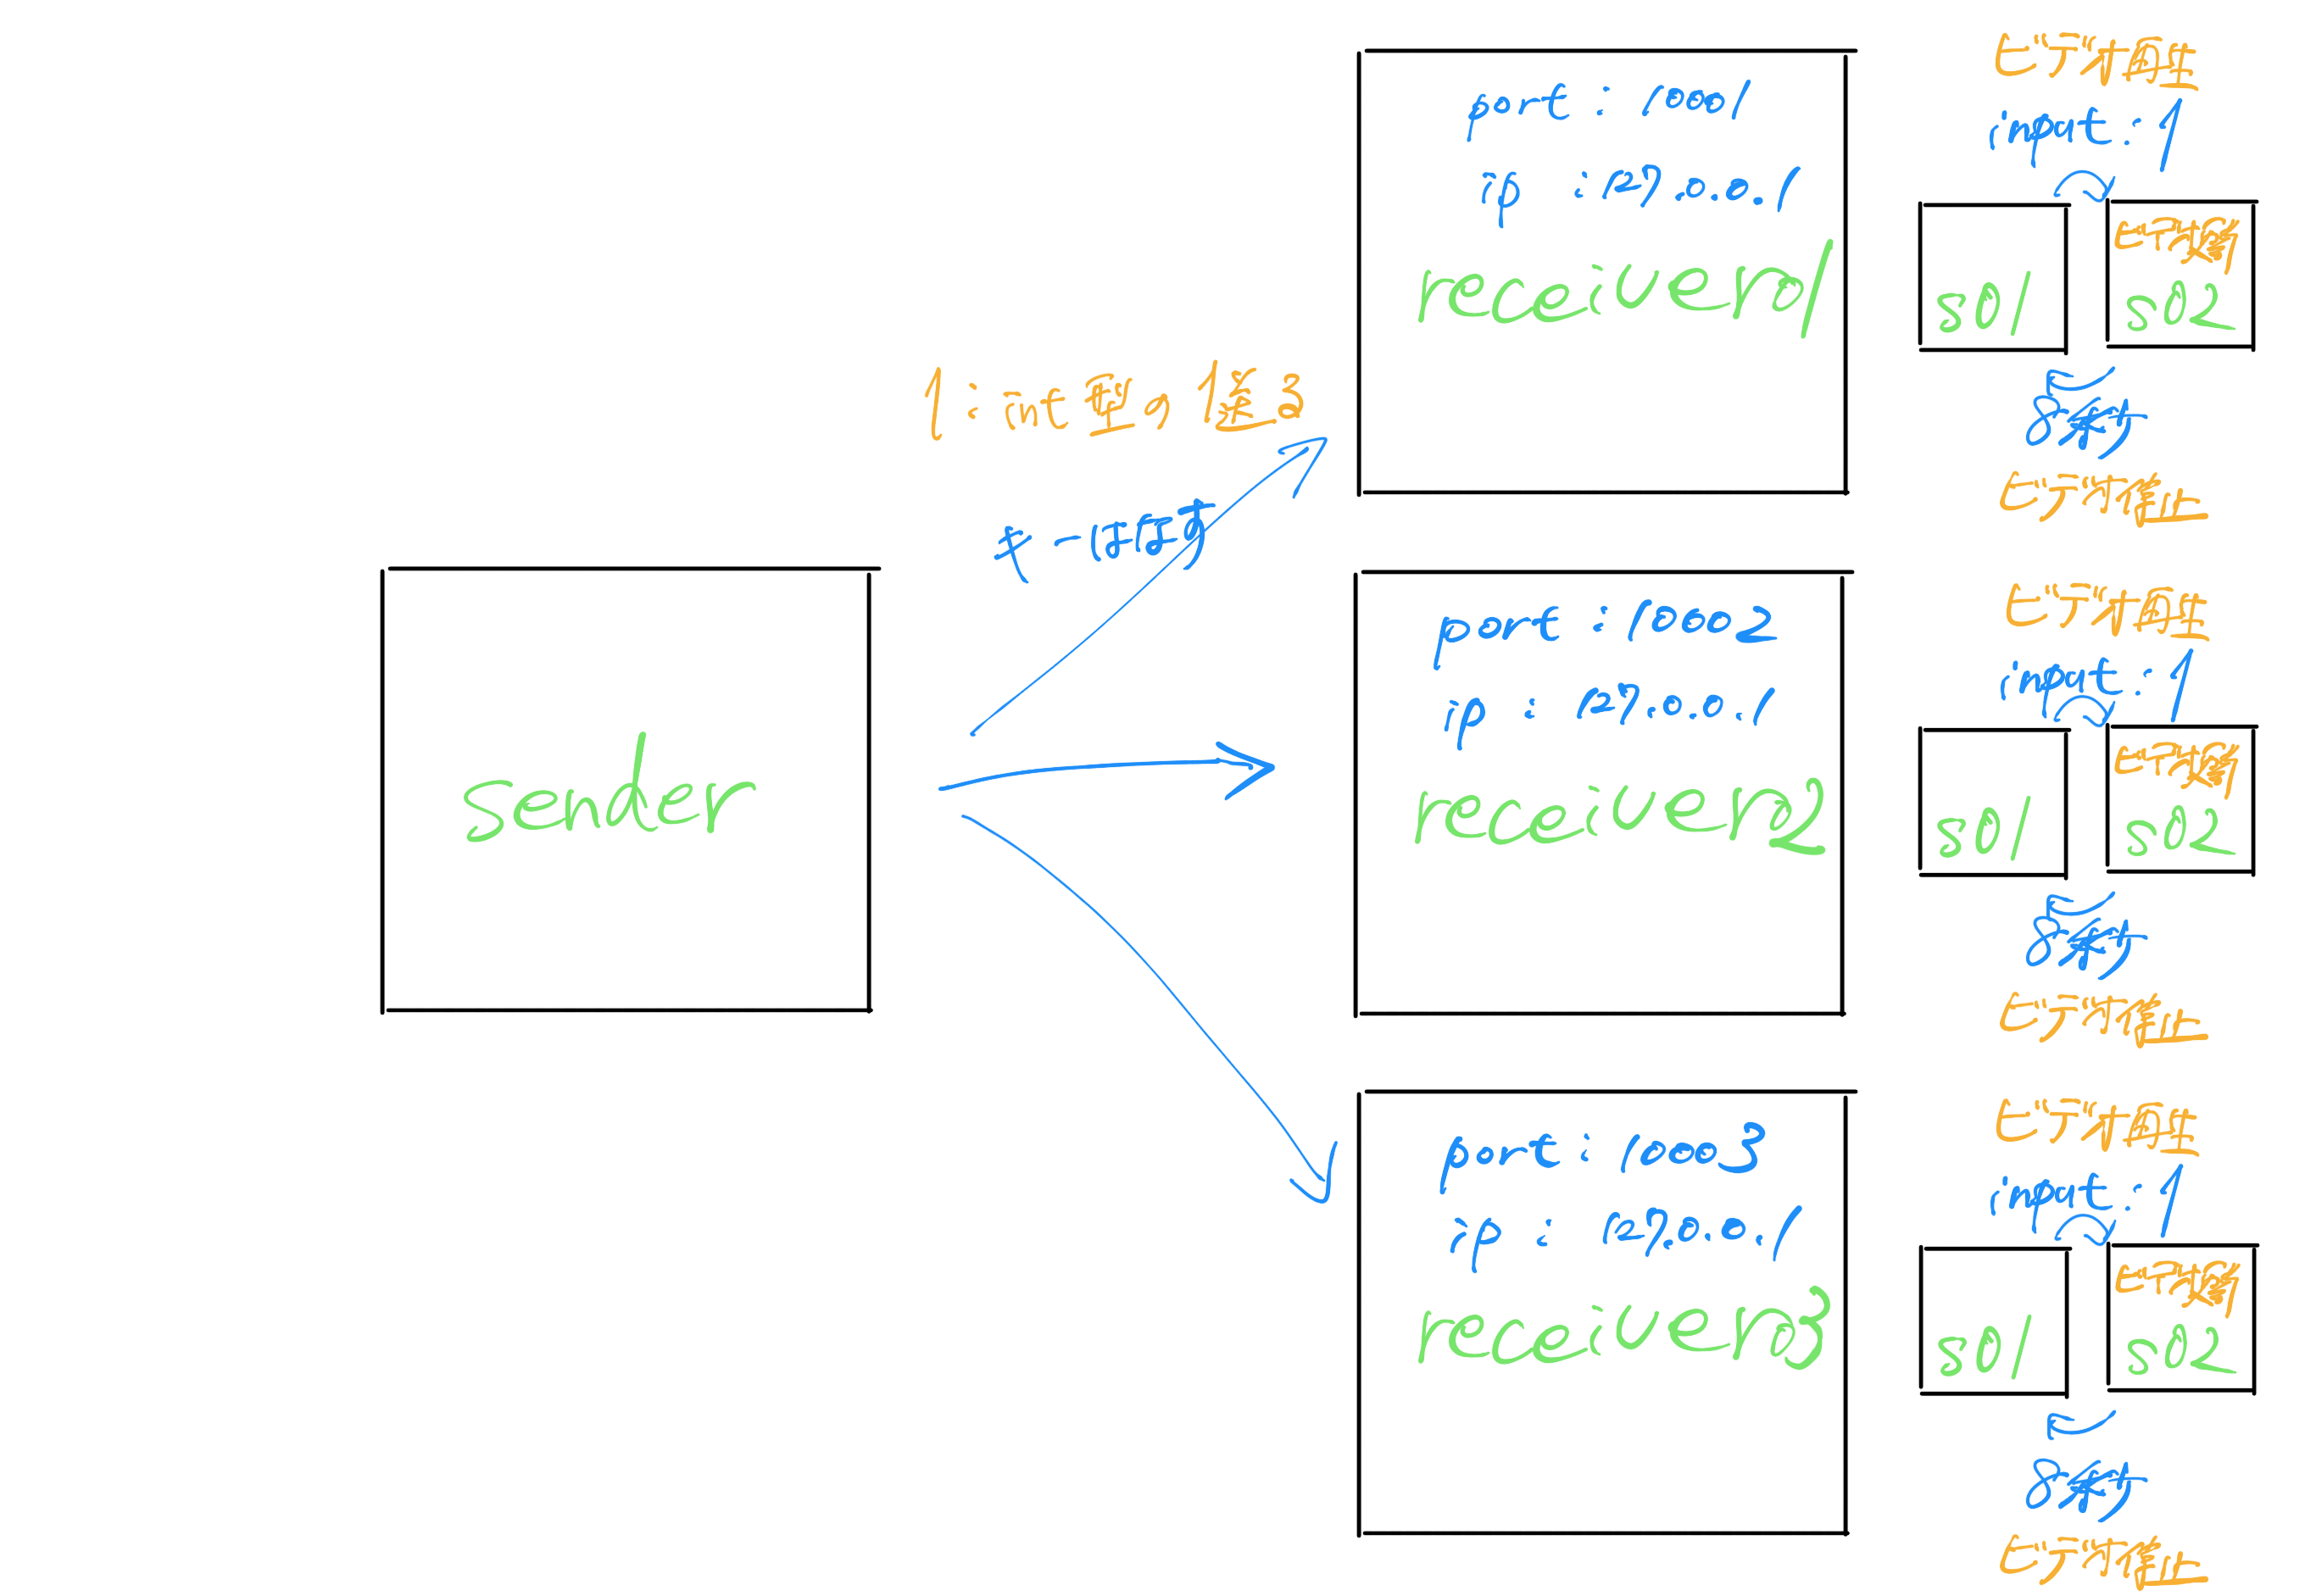
\includegraphics[width=100mm]{images/ws08-1.png}
                    \caption{WS08図解}
                    \label{fig:05}
                \end{figure}
        \end{frame}

    \section{デバイス-pc間通信の作り方}
        \frametitle{Arduinoから値を得る WS09arduino}
        \begin{frame}
            \centering{Arduinoを触りましょう}
        \end{frame}
\end{document}

